\section{最大化$\mathcal{l}(\theta)$的另一种算法}

回到逻辑回归问题,$g(z)$为sigmoid函数,让我们讨论另一种用于最大化$\mathcal{l}(\theta)$的算法。

让我们开始吧,考虑使用牛顿法寻找函数的零点。假设我们有一个函数$f:\mathbb{R}\rightarrow\mathbb{R}$,期望找到一个值$\theta$满足$f(\theta)=0$,其中$\theta \in \mathbb{R}$为实数。牛顿法进行如下操作:
$$
  \theta := \theta - \frac{f(\theta)}{f^\prime(\theta)}
$$
这个方法可以视为,在当前猜测值$\theta$处,通过一个正切于$f$的线性函数近似$f$,以求解该线性函数的零值,然后将下一个$\theta$设置为线性函数的零值。

\begin{figure}
  \begin{center}
    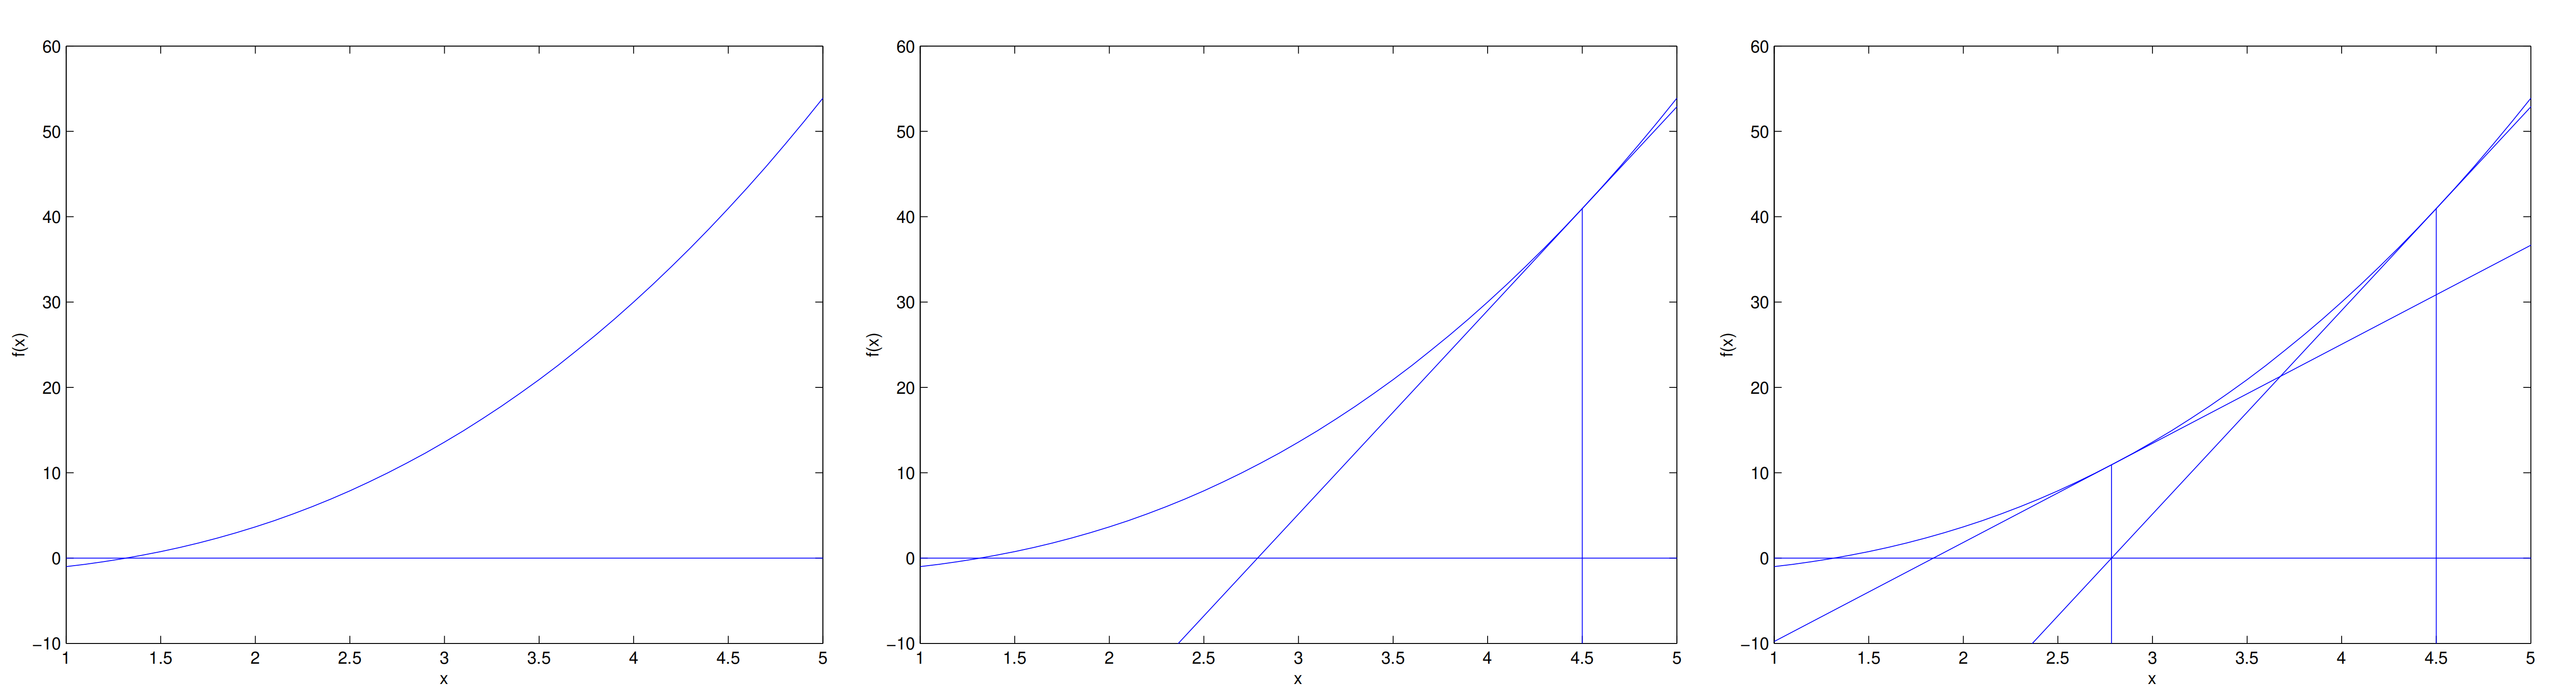
\includegraphics[width=0.9\textwidth]{imgs/2.4_newton.jpg}
  \end{center}
\end{figure}

这里有一张展示牛顿法具体步骤的图片:

在最左边的图片中,可以看到函数$f$与直线$y=0$绘制在一起,我们尝试寻找满足$f(\theta)=0$的$\theta$,能够满足这个目标的$\theta$约为$1.3$。假设我们设置$\theta$为$4.5$初始化此算法。